\documentclass[11pt]{article}
\usepackage[T1,T2A]{fontenc}
\usepackage[utf8]{inputenc}
\usepackage[english,russian]{babel}
\usepackage{graphicx}
\usepackage{amsmath}
\graphicspath {{img/}}

\title{\textbf{Лабораторная работа №2\\<<Исследование процессов в проводных линиях связи>>}}
\author{Перепелица А.А., ККСО-01-19}
\date{Москва, 2022 г.}
\addtolength{\topmargin}{-3cm}
\addtolength{\textheight}{3cm}
\begin{document}
\maketitle
\thispagestyle{empty}
\textbf{Цель работы:} экспериментальное подтверждение волновых процессов в проводных линиях связи, используемых в качестве физической среды при организации каналов передачи данных и приобретение практических навыков постановки и проведения исследований.


\section{ Схема №1: ЛС с потерями в режиме согласованной линии}
\subsection{Перечень элементов, использованных в схемах, с
их краткими характеристиками}
\begin{itemize}
    \item[-] Источник переменного тока (5 В, 500 кГц)
    \item[-] Четырехканальный осциллограф
    \item[-] Двухпроводная ЛС с потерями (50 м, 10 Ом)
    \item[-] Резистор (3.3 кОм)
\end{itemize}

\subsection{Копии окон схемных файлов с позиционными обозначениями}
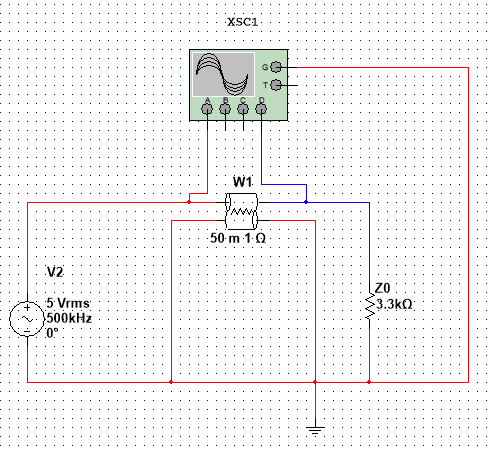
\includegraphics[width=1\linewidth]{img/first.png}
\begin{center}
    Рис.1 Схема ЛС с потерями в режиме согласованной линии.
\end{center}

\subsection{Результаты расчетов и измерений приборами}
Определим значения параметров $Z_0, C, G$:\\

$
Z_0 = \sqrt{\frac{L}{C}} = \sqrt{\frac{11,11\cdot 10^{-6}}{1\cdot 10^{-12}}}\approx 3,3\text{ кОм}\\
L*C = \frac{1}{c^2}=11,11\cdot 10^{-18}\Rightarrow C = \frac{11,11\cdot 10^{-18}}{11,11\cdot 10^{-6}} = 1 \text{ пФ}\\
G = \frac{RC}{L} = \frac{1\cdot 10^{-12}}{11,11\cdot 10^{-6}} = 9\cdot 10^{-8} = 90\cdot 10^{-9} = 90 \text{ нСм/м}\\
$
\newpage
\textbf{Показания осциллографа}
\begin{center}
    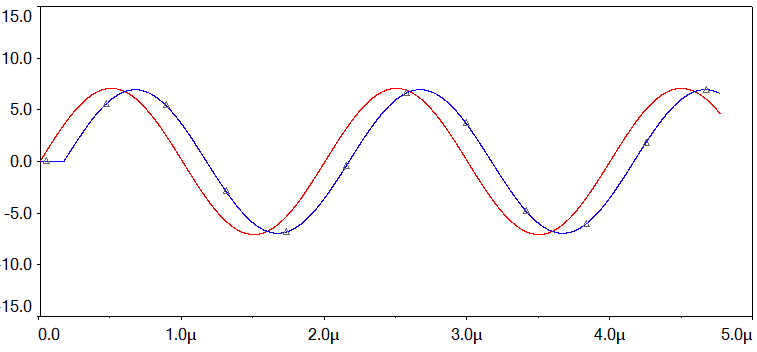
\includegraphics[width=1\linewidth]{img/firstosc1.png}
    Рис.2 Показания осциллографа при частоте 500 кГц.
\end{center}

\begin{center}
    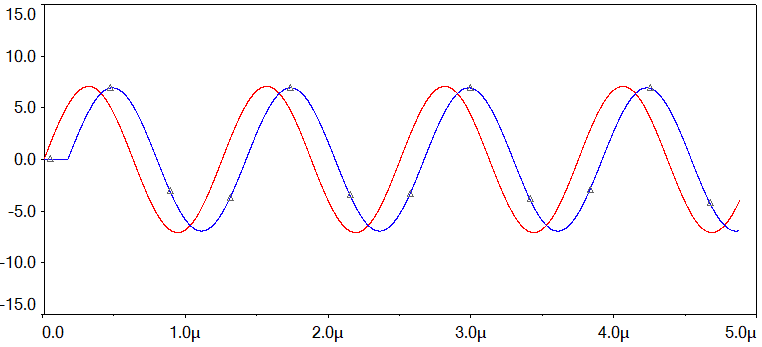
\includegraphics[width=1\linewidth]{img/firstosc2.png}
    Рис.3 Показания осциллографа при частоте 800 кГц.
\end{center}

По графикам видно, что $\tau$ увеличилась. Перестроим модель для $R = 10$ Ом/м.
Для этого поднимем погонную проводимость до $900$ См/м, чтобы выполнялось условие неискажающей линии.
Получим осциллограмму:
\begin{center}
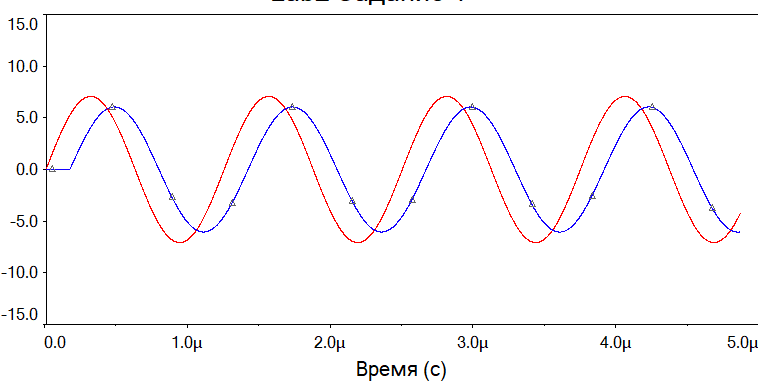
\includegraphics[width=1\linewidth]{img/firstosc3.png}
    Рис.4 Показания осциллографа при  $R = 10$ Ом/м.
\end{center}

Определеим запаздывание выходного сигнала относительно входного на длину линии в режиме бегущей волны:\\
$\beta = 2*\pi*f(T_2-T_1) = 2*\pi*\tau \Rightarrow$ \\ 
$\Rightarrow \beta_1 = 2 * 3.14 * 147 * 10^{-9} = 9,23 * 10^{-6}$\\ 
$\beta_2 = 2 * 3.14 * 163 * 10^{-9} = 10,24 * 10^{-6}$\\ 

Амплитуды входного $U_1$ и выходного напряжения $U_2$:\\
$U_1 = 7,05$В\\
$U_2 = 6,91$В\\
Получим $\alpha$, $\beta l$ и $U$:\\
$\beta = \omega * \sqrt{LC} = 500 * 10^3\sqrt{11,11*10^{-6}* 10^{-12}} \approx 166* 10^{-5}$\\
$\alpha = \sqrt{RG} = \sqrt{10 * 900 * 10^{-9}} = 3 * 10^{-3}$\\
$U(t) = U_i(t)e^{-\alpha l}cos\omega t - \beta l = 7 * e^{-50 * 3 * 10^{-3}} * cos(-166 * 10^{-5} * 50) = 6$В
\newpage
\section{ Схема №2: ЛС с потерями в режиме несогласованной разомкнутой линии}
\subsection{Перечень элементов, использованных в схемах, с
их краткими характеристиками}
\begin{itemize}
    \item[-] Источник переменного тока (5 В, 12 МГц)
    \item[-] Четырехканальный осциллограф
    \item[-] Двухпроводная ЛС с потерями (50 м, 0.001 Ом)
\end{itemize}

\subsection{Копии окон схемных файлов с позиционными обозначениями}
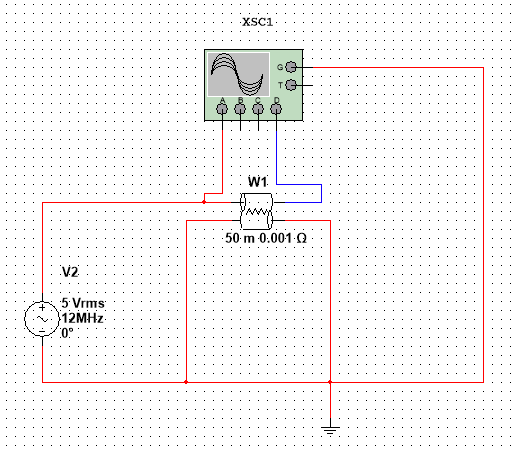
\includegraphics[width=1\linewidth]{img/second.png}
\begin{center}
    Рис.5 Схема ЛС с потерями в режиме несогласованной разомкнутой линии.
\end{center}

\subsection{Результаты расчетов и измерений приборами}
\begin{center}
    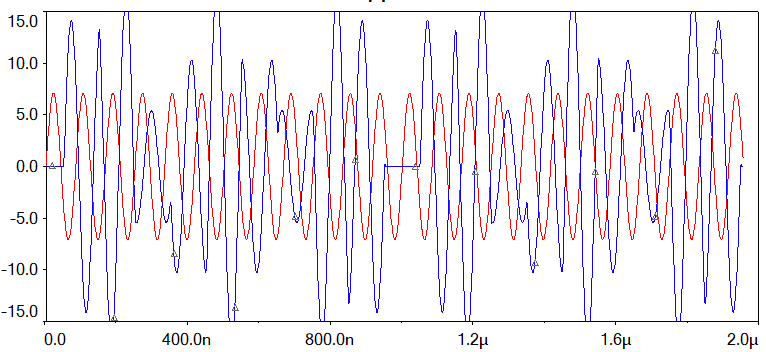
\includegraphics[width=1\linewidth]{img/second1.png}
        Рис.6 Показания осциллографа.
\end{center}
    Запаздывание выходного сигнала относительно входного:\\
    $T_2 - T_1 = 162$нС\\
    Амплитуды входного и выходного напряжений:\\
    $U_i = 6$В\\
    $U = 14$В    
\newpage
\section{ Схема №3: ЛС с потерями в режиме несогласованной замкнутой линии}
\subsection{Перечень элементов, использованных в схемах, с
их краткими характеристиками}
\begin{itemize}    
    \item[-] Источник переменного тока (5 В, 6 Мгц)
    \item[-] Двухпроводная ЛС с потерями (50 м, 0.001 Ом)
    \item[-] Двухпроводная ЛС с потерями (25 м, 0.001 Ом) 2 шт.
    \item[-] Четырехканальный осциллограф
    \item[-] Датчик тока
\end{itemize}

\subsection{Копии окон схемных файлов с позиционными обозначениями}
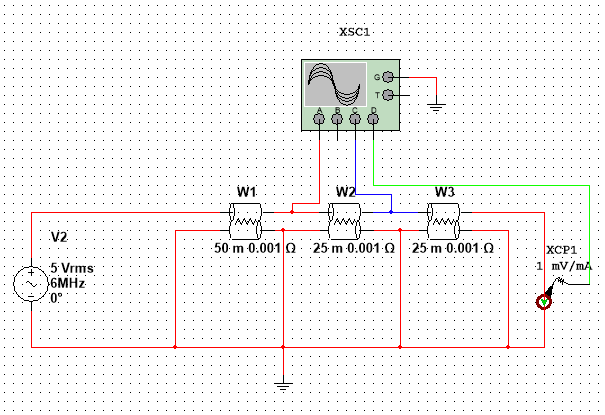
\includegraphics[width=1\linewidth]{img/third.png}
\begin{center}
    Рис.7 Схема ЛС с потерями в режиме несогласованной замкнутой линии.
\end{center}

\subsection{Результаты расчетов и измерений приборами}
\begin{center}
    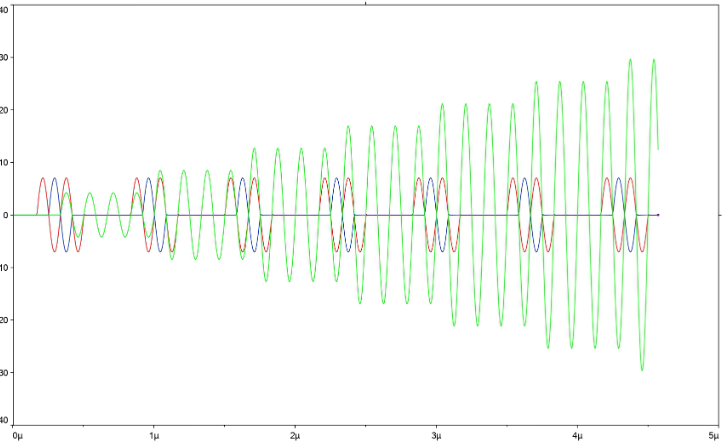
\includegraphics[width=1\linewidth]{img/third1.png}
        Рис.8 Показания осциллографа.
\end{center}
Запаздывание выходного сигнала относительно входного:\\
$T_2 - T_1 = 83$нС\\
Амплитуды входного и выходного напряжений:\\
$U_i = 7$В\\
$U = 7$В
Выходной ток:\\
$I = 800$мА\\

\newpage
\section{ Схема №4: ЛС с потерями в режиме несогласованной нагрузки}
\subsection{Перечень элементов, использованных в схемах, с
их краткими характеристиками}
\begin{itemize}    
    \item[-] Построитель частотных характеристик
    \item[-] Двухпроводная ЛС с потерями (50 м, 1 Ом)
    \item[-] Источник переменного тока (5 В, 500 кГц)
    \item[-] Резистор (0.001 Ом)
    \item[-] Ключ
\end{itemize}

\subsection{Копии окон схемных файлов с позиционными обозначениями}
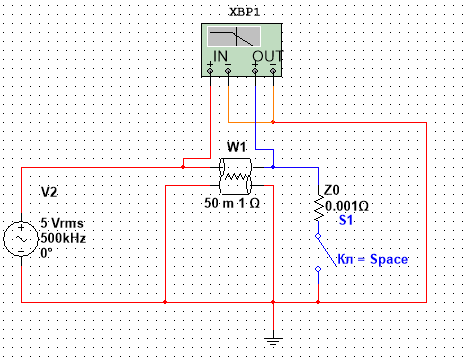
\includegraphics[width=1\linewidth]{img/fourth.png}
\begin{center}
    Рис.9 Схема ЛС с потерями в режиме несогласованной нагрузки.
\end{center}

\subsection{Результаты расчетов и измерений приборами}
\begin{center}
    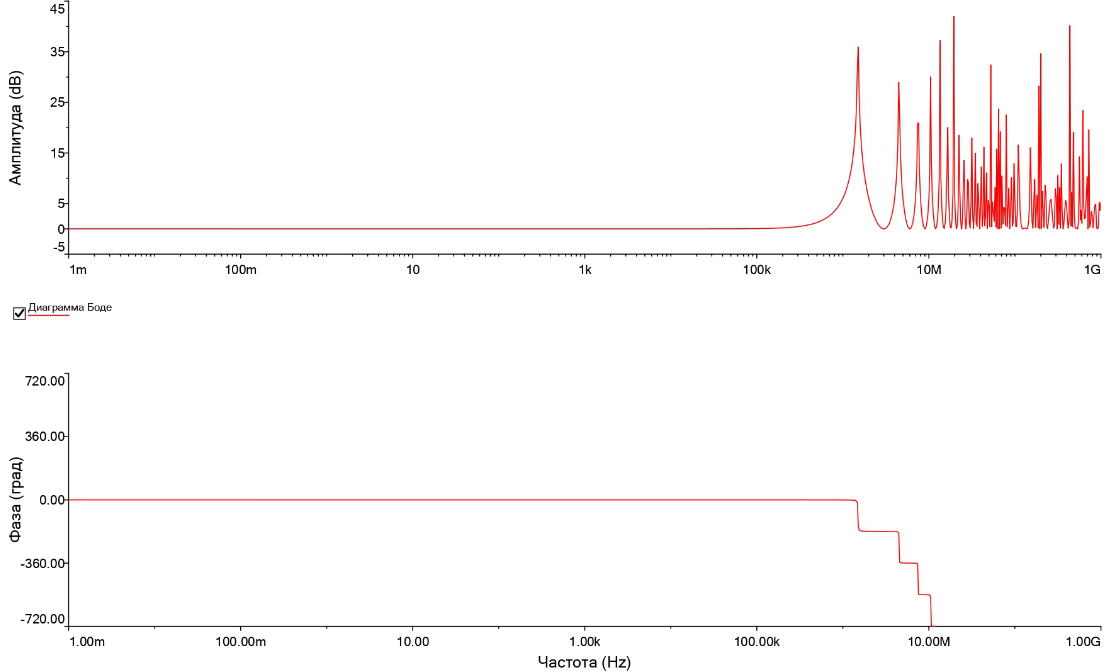
\includegraphics[width=1\linewidth]{img/fourth1.png}
        Рис.10 Показания при разомкнутом ключе.
\end{center}

\begin{center}
    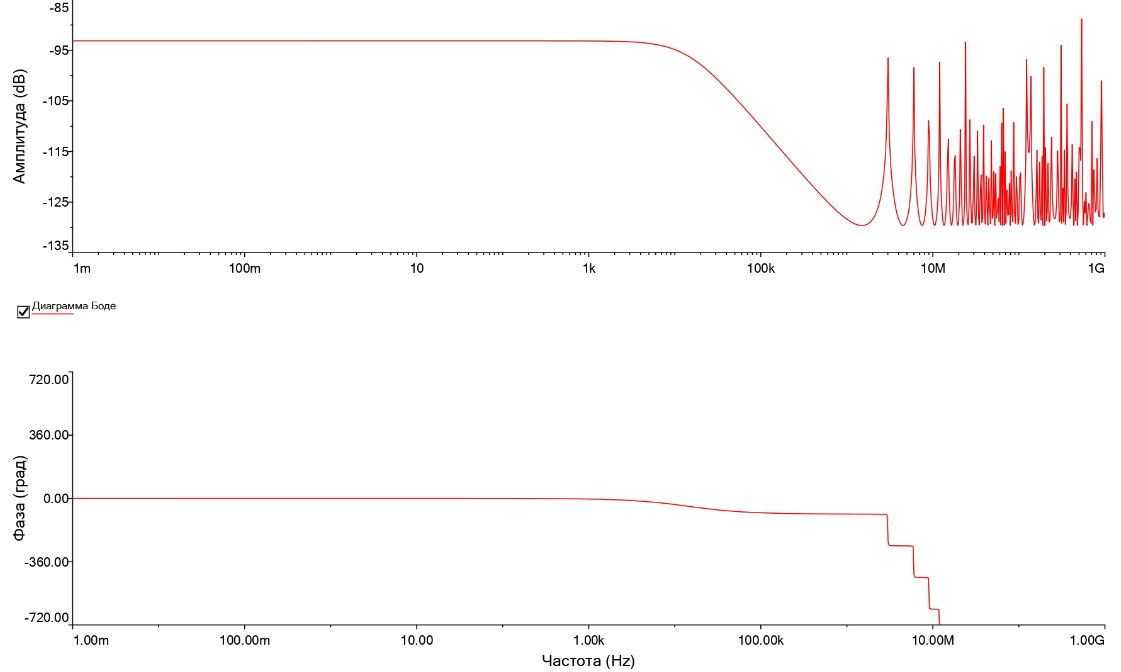
\includegraphics[width=1\linewidth]{img/fourth2.png}
        Рис.11 Показания при замкнутом ключе.
\end{center}


\textbf{Вывод:} в ходе выполнения лабораторной работы мы ознакомились с теорией волновых процессов в проводных линиях связи, исследовали режимы бегущих и стоячих волн.
\end{document}